%%
%% This is file `squelette-rr.tex',
%% generated with the docstrip utility.
%%
%% The original source files were:
%%
%% RR.dtx  (with options: `sample')
%% ********************************************************************
%% Copyright (C) 1997-1999 2004 2006-2010 INRIA/APICS by Jose' Grimm
%% This file may be distributed and/or modified under the
%% conditions of the LaTeX Project Public License, either version 1.3
%% of this license or (at your option) any later version.
%% The latest version of this license is in
%%    http://www.latex-project.org/lppl.txt
%% and version 1.3 or later is part of all distributions of LaTeX
%% version 2003/12/01 or later.
%% An archive of the software can be found at
%%    ftp://ftp-sop.inria.fr/apics/rr-inria

\documentclass[a4paper]{article}
\usepackage[dvipsnames]{color}
\usepackage[latin1]{inputenc} % ou \usepackage[utf8]{inputenc}
\usepackage[T1]{fontenc} % ou \usepackage[OT1]{fontenc}
\usepackage{RR} %,RRthemes}
%\usepackage[dvipsname]{color}
\usepackage{hyperref}
\usepackage{listings}
\usepackage{verbatim}
\usepackage{graphicx}
%%\usepackage[frenchb]{babel} % optionnel
%%
%% date de publication du rapport
\RRdate{November 2011}
%%
%% Cas d'une version deux
%% \RRversion{2}
%% date de publication de la version 2
%% \RRdater{Novembre  2006}
\usepackage{listings}

\usepackage{amssymb}
\usepackage{xspace} 
\usepackage{array} 
\usepackage{multirow}
\newcommand\hyph{\nobreak\hskip0pt-\nobreak\hskip0pt\relax}
\newlength\savedwidth
\newcommand\whline{\noalign{\global\savedwidth
  \arrayrulewidth\global\arrayrulewidth 1.5pt}
  \hline \noalign{\global\arrayrulewidth
  \savedwidth}
}
\newcolumntype{I}{!{\vrule width 1.5pt}}
\renewcommand{\arraystretch}{1.5}

\newcommand{\kaapi}{\textsc{X-Kaapi}\xspace}

%%% For all listing figures
%\definecolor{MyDarkBlue}{rgb}{0.2265625, 0.37109375, 0.80078125}
\definecolor{MyDarkBlue}{rgb}{0.254901960784314,	 0.411764705882353, 0.882352941176471}

\lstset{numbers=left, numberstyle=\tiny, stepnumber=1, numbersep=5pt}
\lstset{commentstyle=\color{blue}}
\lstset{language=C}
\lstset{stringstyle=\ttfamily}
\lstset{ classoffset=1, 
            morekeywords={kaapi,task,data,alloca, declare, reduction, identity, parallel,sync},
            keywordstyle=\color{red}\bfseries
           }
\lstset{ classoffset=2, 
            morekeywords={value,read,write,readwrite,reduction},
%            keywordstyle=\color{red}\bfseries
            keywordstyle=\color{MyDarkBlue}\bfseries
           }
\lstset{ classoffset=3, 
            morekeywords={storage,ld},
%            keywordstyle=\color{red}\bfseries
            keywordstyle=\bfseries
           }
           
\lstset{classoffset=0, showstringspaces=false}



%%
\RRauthor{% les auteurs
 % Premier auteur, avec une note
Fabien Le Mentec%
  % note partag\'ee (optionnelle)
%  \thanks[sfn]{Shared foot note}%
 % \and entre chaque auteur s'il y en a plusieurs
  \and
Thierry Gautier%\thanks{Footnote for second author}%
 % r\'ef\'erence \`a la note partag\'ee
%\thanksref{sfn}
}
%%
%% Ceci apparait sur chaque page paire.
\authorhead{Le Mentec \& Gautier}
%%
\RRtitle{\kaapi~: interface de programmation parall�le}
%% English title
\RRetitle{The \kaapi's Application Programming Interface.
 \Huge{Part II: Parallel Loop}}
%%
\titlehead{The \kaapi's API}
%%
%\RRnote{This is a note}
%\RRnote{This is a second note}
%%
\RRresume{
%Le renouveau de l'utilisation d'un graphe de flot de donn�es pour ex�cutuer les algorithmes par blocs en alg�bre lin�aire est une approche qui vise � garantir la portabilit� des performances des applications sur architecture multi-c\oe urs. L'id�e est d'utiliser une  repr�sentation abstraite des algorithmes en terme de d�pendances de donn�es entre les t�ches ind�pendament de l'algorithme d'ordonnancement qui sera utilis�.

Ce rapport pr�sente le mod�le de programmation \kaapi qui permet d'annonter un programme s�quentiel �crit en C ou C++ par des directives de compilation \texttt{\#pragma} afin de d�crire simplement les t�ches du programme. Un compilateur source � source g�n�re un code qui permet, gr�ce au runtime \kaapi, d'extraire � l'ex�cution ce graphe de flot de donn�es, y compris pour les programmes r�cursifs dont les t�ches seront g�n�r�es r�cursivement. 
}
\RRabstract{%During the past years, dynamically scheduled data flow graphs for tiled algorithms in linear algebra have appeared as a promising way to reach the portability of performance onto several multicore architectures.
%The idea was to describe those algorithms as an abstract data flow graph representation that only encodes tasks and their dependencies independently of the scheduling algorithm, which folds up tasks onto the cores of the target architecture. 
%Reported experimental timings show good performances for linear algebra algorithms where tasks are generated only from nested loops. Nevertheless, all recently proposed frameworks do not consider programs where tasks with data flow dependencies are generated recursively. 

In this report, we present \kaapi's programming model. A parallel \kaapi program is a C or C++ sequential program with code annotation using \texttt{\#pragma} compiler directives. A specific source to source compiler translates \kaapi directives to runtime calls.
}

%%
\RRmotcle{programmation parall�le, graphe de flot de donn�es, ordonnan-cement, \kaapi}
\RRkeyword{parallel computing, data flow graph, scheduling, \kaapi}
%%
%% \RRprojet{Apics}  % cas d'un seul projet
\RRprojets{MOAIS}
%\RRdomaine{3} % cas du domaine numero 1
%\RRthemeProj{moais} % theme du projet Apics
%\RRdomaineProjBis{apics} % domaine du projet Apics
%% \RRdomaineProjBis{pop art} % domaine du projet PopArt
%%
%% \URLorraine % pour ceux qui sont \`a l'est
%% \URRennes  % pour ceux qui sont \`a l'ouest
%% \URRhoneAlpes % pour ceux qui sont dans les montagnes
%% \URRocq % pour ceux qui sont au centre de la France
%% \URFuturs % pour ceux qui sont dans le virtuel
%% \URSophia % pour ceux qui sont au Sud.
%%
%% \RCBordeaux % centre de recherche Bordeaux - Sud Ouest
%% \RCLille % centre de recherche Lille Nord Europe
%% \RCParis % Paris Rocquencourt
%% \RCSaclay % Saclay \^Ile de France
\RCGrenoble % Grenoble - Rh\^one-Alpes
%% \RCNancy % Nancy - Grand Est
%% \RCRennes % Rennes - Bretagne Atlantique
%\RCSophia % Sophia Antipolis M\'editerran\'ee

%%
\begin{document}
%%
%\makeRR   % cas d'un rapport de recherche
\makeRT % cas d'un rapport technique.
%% a partir d'ici, chacun fait comme il le souhaite


\tableofcontents

% Environment overview
%
\newpage
\section{Introduction}
\paragraph{}
XKAAPI is a runtime exporting a set of functions to create and schedule computation tasks.
Scheduling relies on the workstealing paradigm where a processor steals computation tasks
as it becomes idle. Among the programming models, XKAAPI allows for adaptive tasks creation,
ie. tasks that are created on demand by splitting a work set.
\paragraph{}
Programming adaptive tasks is not easy since the exported interface requires knowledge
about the runtime inner workings. As a result, we implemented automatic loop parallelisation
in the KACC compiler, that only requires the user to annotate the corresponding code with
\textit{\#pragma} directives.
\paragraph{}
This report details the current implementation status, and can be used as a base for futur
work. Benchmarks and example applications are also included. It concludes by giving ingishts
on issues that remain to be addressed and directions for futur studies.

\newpage
\section{Automatic loop parallelisation}

\subsection{Loop structure constraints}
\subsubsection{General form}
\paragraph{}
A classical C/C++ \textit{for} loop construct has the following form:\\

\begin{small}
\lstset{commentstyle=\color{blue}}
\lstset{language=C}
\begin{lstlisting}[frame=tb]
for (initialization; condition; increment) body ;
\end{lstlisting}
\end{small}

\paragraph{}
With some constraints, this is the kind of loop automatic parallelisation
is applied to. A user informs KACC to parallelise a loop by annotating it
with a \textit{\#pragma kaapi loop} directive:\\

\begin{small}
\lstset{commentstyle=\color{blue}}
\lstset{language=C}
\begin{lstlisting}[frame=tb]
#pragma kaapi loop
for (initialization; condition; increment) body ;
\end{lstlisting}
\end{small}

\subsubsection{Initialization clause}
\paragraph{}
The \textit{initialization} clause is a standard statement. Note that it
can be outside the loop:\\

\begin{small}
\lstset{commentstyle=\color{blue}}
\lstset{language=C}
\begin{lstlisting}[frame=tb]
initialization;
#pragma kaapi loop
for (; condition; increment) body ;
\end{lstlisting}
\end{small}

\subsubsection{Condition clause}
\paragraph{}
A valid clause is a testing statement of the form:\\
\begin{small}
\lstset{commentstyle=\color{blue}}
\lstset{language=C}
\begin{lstlisting}[frame=tb]
lhs binary_operator rhs
\end{lstlisting}
\end{small}
\paragraph{}
An \textit{binary\_operator} is valid if it belongs to the following list:
\begin{center} $<$, $<=$, $>$, $>=$, $!=$ \end{center}
Note that the corresponding C++ operators are considered valid.
\paragraph{}
As an arbitrary choice, the \textit{condition} left hand side is always defined to be the loop
\textit{iterator} name. There is currently no way to override this.

\subsubsection{Increment clause}
\paragraph{}
The \textit{increment} clause is a list of one or more variable updating expressions. Note that
there should at least be one expression updating the \textit{iterator} variable. An expression is
valid if it has one of the following form:\\
\begin{small}
\lstset{commentstyle=\color{blue}}
\lstset{language=C}
\begin{lstlisting}[frame=tb]
var = var op rhs;
var += rhs; // eq. var -= rhs
++var; // eq. --var
var++; // eq. var--
\end{lstlisting}
\end{small}

\paragraph{}
For instance, below is a valid construct:\\
\begin{small}
\lstset{commentstyle=\color{blue}}
\lstset{language=C}
\begin{lstlisting}[frame=tb]
#pragma kaapi loop
for (initialization; condition; i += 2, j -= 4, ++k) body ;
\end{lstlisting}
\end{small}

\paragraph{}
The set of \textit{affine} variables is built by gathering all the updated variables. In the
above example, the set is thus $\{i, j, k\}$. It is important to note that a variable in this set
cannot be updated by the loop body.

\subsubsection{Iteration direction}
\paragraph{}
The iteration can be \textit{forward} or \textit{backward}, defining its direction. The direction
is important since it is used to determine the iteration \textit{range}. An increasing (resp. decreasing)
operator in the \textit{increment} clause means a \textit{forward} (resp. \textit{backward}) iteration.\\
\begin{small}
\lstset{commentstyle=\color{blue}}
\lstset{language=C}
\begin{lstlisting}[frame=tb]
/* ++ is an increasing operator, forward iteration */
for (initialization; condition; ++i) body ;

/* -= is a decreasing operator, backward iteration */
for (initialization; condition; i -= 2) body ;
\end{lstlisting}
\end{small}

\subsubsection{Iteration interval}
\paragraph{}
The iteration \textit{count} is always defined by the formula:
\begin{center}
  $iteration\_count = \Bigl\lceil \frac{hi\_bound - lo\_bound}{iterator\_increment} \Bigr\rceil$
\end{center}
where:
\begin{itemize}
\item \textit{initial\_value} is the iterator value upon loop entry,
\item if this is a \textit{forward} iteration, \textit{hi\_bound} is set to the \textit{condition}
clause right hand side and \textit{lo\_bound} is set to \textit{initial\_value},
\item if this is a \textit{backward} iteration, \textit{hi\_bound} is set to the \textit{initial\_value}
and \textit{lo\_bound} is set to the \textit{condition} clause right hand side,
\item 1 is added according to the \textit{condition} strictness.
\end{itemize}
Thus the iteration spans the following interval:
\begin{center}
  $\Bigl[ initial\_value, initial\_value + iteration\_count \Bigr[$
\end{center}

\subsection{Supported pragma clauses}
\paragraph{}
To drive KACC during loop parallelisation, a set of clauses can be append to the
\textit{\#pragma kaapi loop} directive. Here is the list of currently supported clauses:
\begin{itemize}
  \item \textit{reduction(reduction\_identifier: variable\_name , ...)}: it works similarly
    to DFG task reduction. Refer to the compiler manual for more information.
\end{itemize}

\subsection{Notes}
\paragraph{}
A current important limitation is that none of the variables gets updated at the end
of the loop, with the exception of variables present in reduction clauses. A missing
\textit{output} clause should be implemented.
\paragraph{}
There is implicitely assumed that the working sequences have a random access iterators
semantic.

\subsection{Examples}
\paragraph{}
3 source code listings are provided as examples:
\begin{itemize}
\item \textit{for\_each}: apply a function to the elements of a sequence,
\item \textit{accumulate}: sum all the sequence elements into a scalar,
\item \textit{inner\_product}: compute the dot product of 2 vectors.
\end{itemize}

\pagebreak
\begin{small}
\lstset{commentstyle=\color{blue}}
\lstset{language=C}
\begin{lstlisting}[frame=tb, caption={for\_each}]
/* iterate using an index
 */
static void for_each(double* v, unsigned int n)
{
  unsigned int i;
#pragma kaapi loop
  for (i = 0; i < n; ++i) v[i] += 1;
}

/* iterate using the pointer
 */
static void for_each(double* v, unsigned int n)
{
#pragma kaapi loop
  for (; n > 0; --n, ++v) *v += 1;
}

\end{lstlisting}
\end{small}

\begin{small}
\lstset{commentstyle=\color{blue}}
\lstset{language=C}
\begin{lstlisting}[frame=tb, caption={accumulate}]
/* define a reduction function
 */
static void reduce_sum(double* lhs, const double* rhs)
{
  *lhs += *rhs;
}

/* associate an id to the reduction function
 */
#pragma kaapi declare reduction(reduce_sum_id: reduce_sum)

/* accumulate algorithm using a reduction clause
 */
static double accumulate(const double* v, unsigned int n)
{
  unsigned int i;
  double sum = 0;
#pragma kaapi loop reduction(reduce_sum_id:sum)
  for (i = 0; i < n; ++i) sum += v[i];
  return sum;
}
\end{lstlisting}
\end{small}

\pagebreak
\begin{small}
\lstset{commentstyle=\color{blue}}
\lstset{language=C}
\begin{lstlisting}[frame=tb, caption={inner\_product}]
/* define a reduction function
 */
static void reduce_sum(double* lhs, const double* rhs)
{
  *lhs += *rhs;
}

/* associate an id to the reduction function
 */
#pragma kaapi declare reduction(reduce_sum_id: reduce_sum)

/* accumulate algorithm using a reduction clause
 */
static double inner_product( const double* u, 
                             const double* v, 
                             unsigned int n )
{
  double sum = 0;
#pragma kaapi loop reduction(reduce_sum_id:sum)
  for (; n > 0; --n, ++u, ++v) sum += (*u) * (*v);
  return sum;
}
\end{lstlisting}
\end{small}

\newpage
\section{Synthetic benchmark: sequence iteration}

\paragraph{}
Figure \ref{foreach_speedups} shows the speedup of a program applying a given function to
all the elements of a sequence, such as:
\begin{center}
  $v[i] = f_{nn}(v[i]);$
\end{center}
The applied function basic operation count, \textit{NN}, is indicated as a subscript in the graph legend.

\paragraph{}
Information about the experiment:
\begin{itemize}
\item The host is IDFREEZE,
\item The command line uses \textit{numactl --interleave=all},
\item The speedup is computed relatively to the sequential program,
\item The sequence size is 4 * 1024 * 1024 double.
\end{itemize}

\begin{figure}[!hb]
\centering
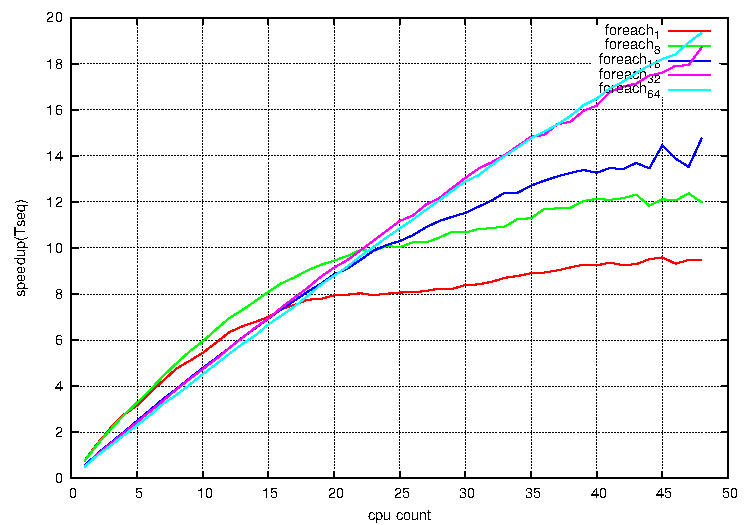
\includegraphics[keepaspectratio=true, width=\linewidth]{../graphs/foreach_speedups.pdf}
\caption{$foreach_{NN}$ where NN the operation count}
\label{foreach_speedups}
\end{figure}

As we can see, $\frac{Tseq}{T1}$ is low and decreases as the operation count increases. Without entering the details,
this is due to the generated machine code, and has only very little to do with runtime related overheads. It thus
seems important to have a look at the speedup for the same experience, but measured against the parallel program with
1 processor. This is shown in Figure \ref{foreach_speedups_t1}.

\begin{figure}[!ht]
\centering
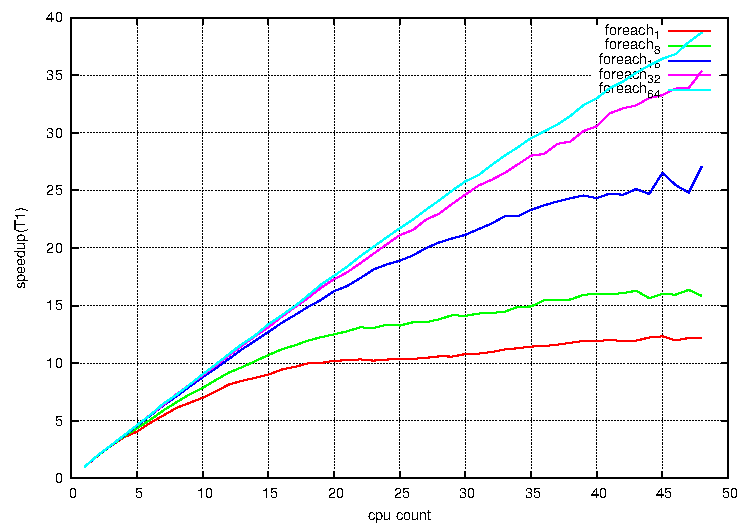
\includegraphics[keepaspectratio=true, width=\linewidth]{../graphs/foreach_speedups_t1.pdf}
\caption{$foreach_{NN}$ where NN the operation count}
\label{foreach_speedups_t1}
\end{figure}

\newpage
\section{Synthetic benchmark: sequence accumulation}

\paragraph{}
Figure \ref{accumulate_large} shows the speedup of a program accumulating the
elements of a sequence into a single reduction variable, such as:
\begin{center}
  $\sum_{i=0}^n v[i] * v[i] * ... * v[i]$
\end{center}
The multiplication count, \textit{NN}, is indicated as a subscript in the graph legend.

\paragraph{}
Information about the experiment:
\begin{itemize}
\item The host is IDFREEZE,
\item The command line uses \textit{numactl --interleave=all}
\item The speedup is computed relatively to the sequential program,
\item The sequence size is 4 * 1024 * 1024 double.
\end{itemize}

\begin{figure}[!ht]
\centering
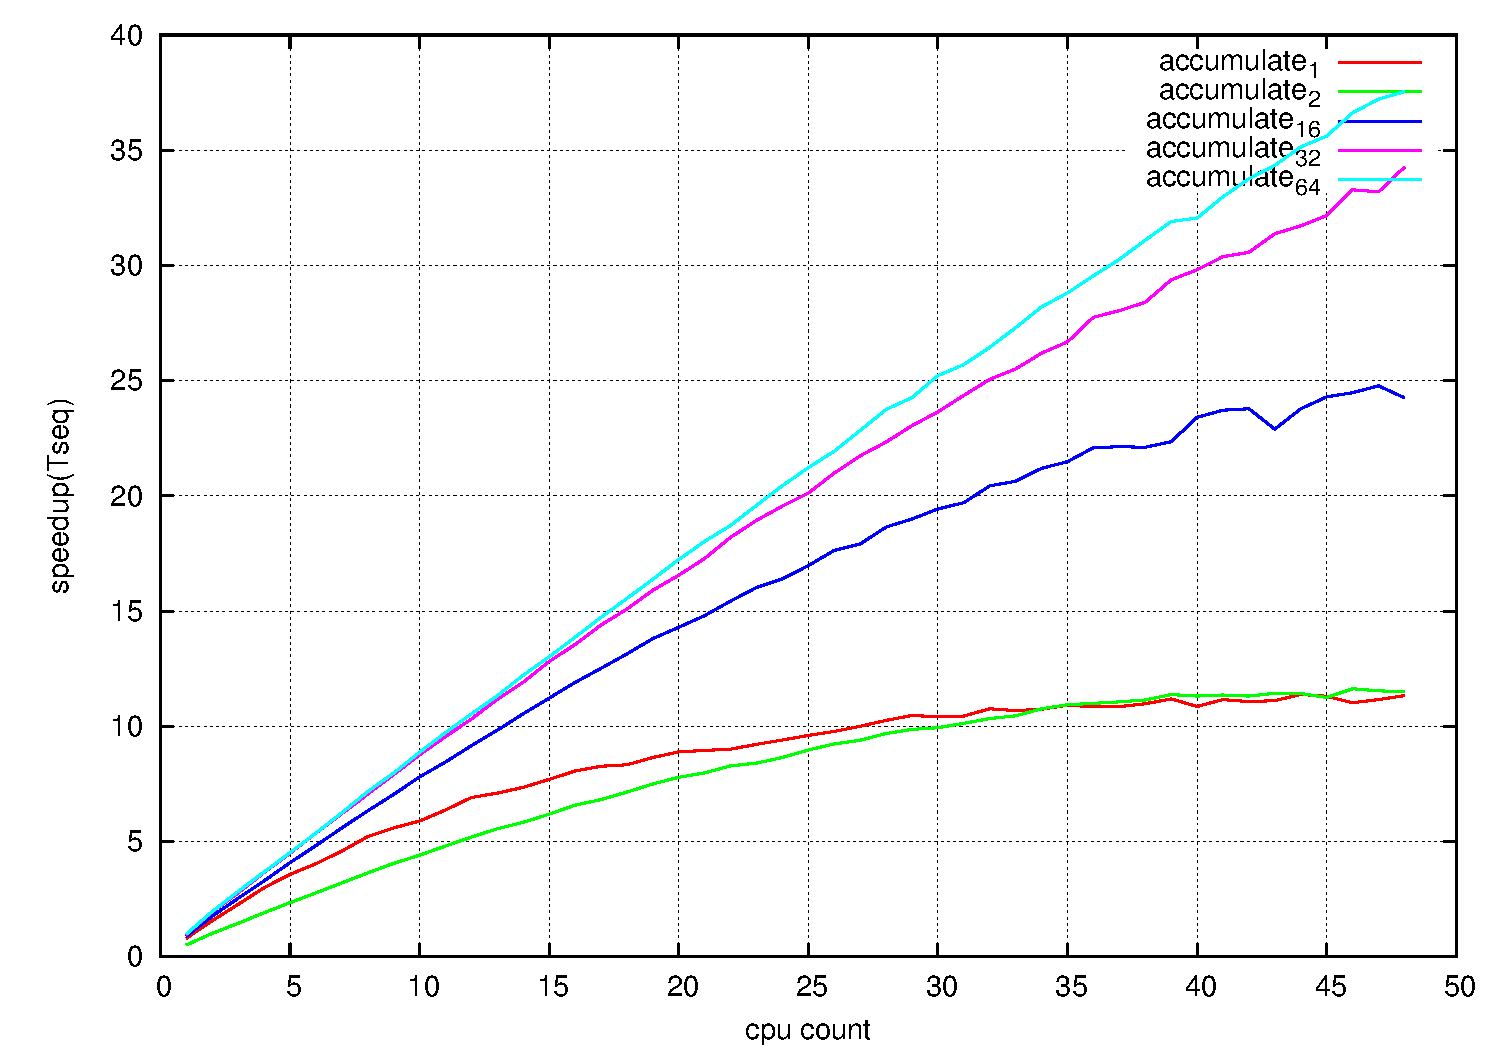
\includegraphics[keepaspectratio=true, width=\linewidth]{../graphs/accumulate_large_sequence_speedups.pdf}
\caption{$accumulate_{NN}$ where NN the operation count}
\label{accumulate_large}
\end{figure}

\paragraph{}
As expected, we see that the program scales more as the operation count increases
(ie. increasing arithmetic over memory operation ratio).

\paragraph{}
Note that the sequential program performs better than the parallel one 1 core.
This penalty is inversely proportionnal to the operation count per sequence
element, and is non negligeable if the count is low. We emphasis that the XKAAPI
runtime overhead is minor in this performance issue. Here are the reasons:
\begin{itemize}
  \item Analysing the generated assembly code shows that a less efficient
    register usage is done, resulting in more memory operation per iteration.
    This has a dramatic impact on performance if the operation count is low.
  \item KACC adds one arithmetic operation per iteration of a parallel loop.
  \item Extracting from the XKAAPI workqueue incurs overhead. In this benchmark,
    we should note that work extraction costs are largely amortized.
\end{itemize}

\newpage
\section{OpenDE library}

\subsection{Overview}
\paragraph{}
OpenDE is a rigid body dynamics simulation opensource library. The website is available at:
\begin{center}
  \textit{http://www.ode.org}
\end{center}

\paragraph{}
This is a real world application not written with parallelism in mind. The C/C++ code does not
make a use of heavy or complicated syntaxic constructs, and is easily parsed by the source to source
framework. Most of the \textit{for} loop structures are suitable for automatic parallelisation.
Thus, it is a good candidate to apply our work on.
\paragraph{}
A GIT repository tracking original code modifications is available here:
\begin{center}
  https://github.com/texane/opende\_kaapi
\end{center}

% TODO
%
% \subsection{Required code modifications}
% \begin{itemize}
%   \item packed body vector
%   \item integral sequences
%   \item output variables
% \end{itemize}
%
% TODO

\subsection{Preprocessing step}
\paragraph{}
In this work, we focused on the \textit{step.cpp} file. It contains a function
\textit{dInternalStepIsland\_x2} that gets called at each simulation time step.
This function is divided into several smaller steps. Among other things, those
steps perform one or more iterations on the body vector.
\paragraph{}
In the example used for the benchmark, the \textit{preprocessing} step consumes
nearly 37\% of an iteration time. From now on, we only focus on it. It consists
of the following pseudocode:
\pagebreak
\begin{small}
\lstset{commentstyle=\color{blue}}
\lstset{language=C}
\begin{lstlisting}[frame=tb]
foreach (body)
{
  body->tag = i;
}

foreach (body)
{
  compute_inverse_inertia_tensor(body);
  if (body->isGiroscopic)
  {
    compute_inertia_tensor(body);
    compute_rotational_force(body);
  }
}

foreach (body)
{
  add_gravity(body);
}
\end{lstlisting}
\end{small}

\end{document}

%%%%%% Pour apr�s
%%%%%% 
\subsection{Benchmarks}
\paragraph{}
Figure \ref{opende_speedups} shows the speedup of the \textit{preprocessing} step of the
\textit{demo\_step} application shipped with OpenDE. The code can be retrieved on the
\textit{opende\_kaapi} repository, commit:
\begin{center}
  bb96672ada398f0f7e39d03a091d8195133895f3
\end{center}

\paragraph{}
Information about the experiment:
\begin{itemize}
\item The host is IDKOIFF (OpenGL related problems on IDFREEZE),
\item The command line uses \textit{numactl --interleave=all},
\item The speedup is computed relatively to the sequential program,
\end{itemize}

\begin{figure}[!ht]
\centering
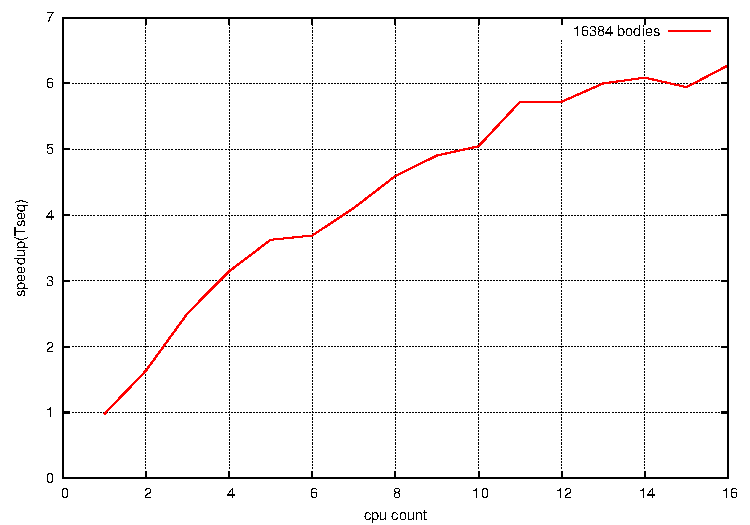
\includegraphics[keepaspectratio=true, width=\linewidth]{../graphs/opende_speedups.pdf}
\caption{opende speedups}
\label{opende_speedups}
\end{figure}

\paragraph{}
Figure \ref{opende_speedups} shows that the speedup is limited. 3 reasons may explain that:
\begin{itemize}
  \item memory cache related issues,
  \item workstealing engine issues,
  \item the problem size is too small.
\end{itemize}

\paragraph{}
Since XKAAPI does not yet handle memory affinity, a work interval is unlikely to be distributed to the core
that worked on it in the previous algorithm. Consequently, having multiple consecutive loops instead of one
may have cache related effect. More importantly, the probability for a processor $P_i$ to steal a memory word
$M_j$ decreases as the processor count increases. Thus, cache effects are related to the processor count.\\
To verify this claim, we could have increased the rigid body count to make the stolen interval bigger than
the cache. Unfortunately, OpenDE crashes as we allocate larger body vectors.\\
We chose a different approach: merging the different loops into a single one, such that the \textit{preprocessing}
step pseudo code becomes:\\
\begin{small}
\lstset{commentstyle=\color{blue}}
\lstset{language=C}
\begin{lstlisting}[frame=tb]
foreach (body)
{
  body->tag = i;
  compute_inverse_inertia_tensor(body);
  if (body->isGiroscopic)
  {
    compute_inertia_tensor(body);
    compute_rotational_force(body);
  }
  add_gravity(body);
}
\end{lstlisting}
\end{small}
The resulting speedup graph is shown in Figure \ref{opende_merged_speedups}

\begin{figure}[!hb]
\centering
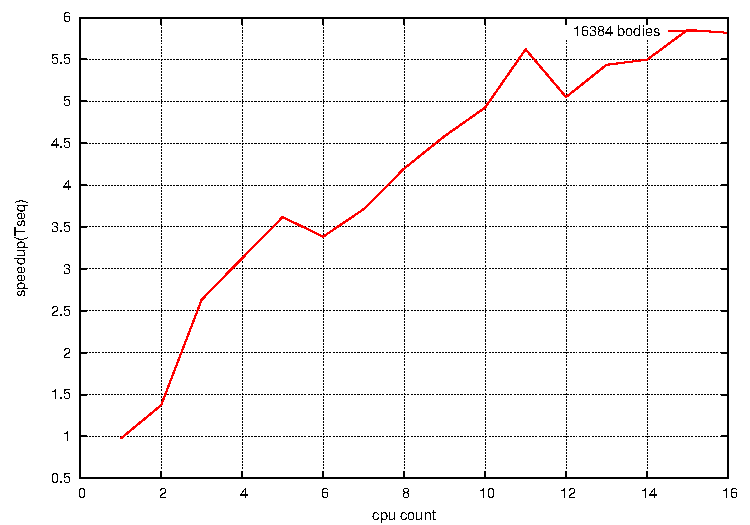
\includegraphics[keepaspectratio=true, width=\linewidth]{../graphs/opende_merged_speedups.pdf}
\caption{single loop speedup}
\label{opende_merged_speedups}
\end{figure}
This graph clearly invalids our claim regarding cache effects.

\paragraph{}
Another explanation could lie in the workstealing engine. However, we did not observe any
incorrect behavior in the previous synthetic experiments. We thus conclude that the speedup
limiting factor is the problem size.

\subsection{Future work}
\paragraph{}
Due to the lack of time, no significant progress has been made on the LCP solver. As
the number of joints and contacts increase in the scene, the time spent solving constraint
equations becomes largely dominant. The code is entierly written by hand, as are all the
matrix related operations. Thus, it is not possible to use a parallel linear algebra library.

\newpage
\section{Conclusion and futur work}

\subsection{Conclusion}
\paragraph{}
Automatic loop parallelisation can be useful to parallelize existing sequential
applications with relatively few code modifications. There are still strong
constraints on the loop structure, as well as performance issues on strongly
memory bound, iterative applications. The remaining subsections list a set of
directions to improve the current work.

\subsection{Automatic grain tuning}
\paragraph{}
There is a size below which the problem should not be splitted anymore, since
the runtime costs become more important than the actual task processing ones.
Currently, a threshold is set constant and large enough to armotize the runtime
related costs for most problems. This code can be found in:
\begin{center}
  \textit{\$XKAAPI/src/misc/kaapi\_splitter.c}
\end{center}
While it works on the tested problems, a constant threshold relates to a size which
is independant of the actual task processing costs. It may prevent a small sized task
to be split, while it actually has large processing costs from which parallelism could
be extracted. Some work is needed to make the split criteria more flexible.

\subsection{Memory affinity splitter}
\paragraph{}
Currently, strongly memory bound iterative applications suffer from performance issues.
There are already works in progress to address memory affinity related problems. A binding
attribute is present but not yet exploited in the XKAAPI runtime. Recently, Damien Leone
worked on splitting policy that conserve memory affinity information over loop iteration.

\subsection{Missing loop pragma clauses}
\paragraph{}
Currently, the compiler automatically guesses the loop parameters as long as the loop
is expressed in a suitable form. There is yet no way for the user to override the compiler
decisions. To do so, a set of pragma clauses should be added, for instance:
\begin{itemize}
  \item \textit{affine(variable\_names)}: defines a set of variables which are considered affine
  \item \textit{output(variable\_names)}: defines a set of variables which must be updated at the
    end of the loop. Currently, no variable is updated as a loop terminates.
  \item \textit{iterator(variable\_name)}: defines which variable drives the loop execution.
\end{itemize}

\subsection{Extend to multi level loops}
\paragraph{}
Currently, KACC only targets one level loops. This is an obvious limitation for applications
working on multidimensionnal structures, such as image processing or linear algebra. In the
case of image processing kernels, a solution is to linearize the 2d domain.

\subsection{Atomic pragma clause}
\paragraph{}
Even if this can leads to scalability issues, atomic operations can be useful when
parallelising a sequential program. An \textit{atomic} directive could be added before
statements or variable declarations. Note that the implementation should not be constrained
by the hardware atomic instruction availability or applicability. For instance, if the target
variable is not a machine word, a lock or even a critical section may be used to implement
atomicity.

\subsection{FORTRAN language support}
\paragraph{}
KACC will eventually be used by projects written in FORTRAN (ie. EUROPLEXUS). While the
ROSE source to source framework support this language, KACC has not yet been tested on
Fortran source code files.

\subsection{Large project support (NOT RELATED TO ADAPTIVE LOOPS)}
\paragraph{}
There are some limitations in the source to source compilation framework that prevent
large C++ projects to be compiled by KACC (ie. SOFA). The limitations include namespace
resolution and performance issue, making the compilation process ways too slow. Those
problems need to be solved.

\subsection{KACC driver integration (NOT RELATED TO ADAPTIVE LOOPS)}
\paragraph{}
Ideally, we would like to replace a project compiler (ie. GCC) by KACC. It currently
in most cases, but features are still missing. For instance, we would like to filter
the KACC processed files, by adding a \textit{.kacc\_filter} file list in each subdirectories.

\end{document}
